% !TeX spellcheck = fr_FR
\chapter{Théorème et formule intégrale de Cauchy}


\section{Intégration complexe}

\subsection{Définitions et notations}

\begin{definition}[10.1, p.73]\hfill
\begin{enumerate}[label=\arabic{enumi})]
    \item
    $\Gamma \subset \C$ est une \textbf{courbe simple régulière} s'il existe un intervalle $[a,b] \subset \R$ et une fonction $\gamma: \begin{array}{ccl} [a,b] & \longrightarrow & \C\\ t & \longmapsto & \gamma(t) = \gamma_1(t) + i\gamma_2(t)\end{array}$ telle que:
    
    \begin{itemize}
    \item $\Gamma = \gamma([a,b])$, la courbe $\Gamma$ est l'image de $\gamma$
    \item $\gamma(t_1) = \gamma(t_2) \implies t_1 = t_2 \enspace \forall t_1,t_2 \in [a,b[$
    \item $\gamma \in C^1\left([a,b]\right)$
    \item $\module{\gamma'(t)} = \left[\gamma_1'(t)^2 + \gamma_2'(t)^2\right]^\frac{1}{2} \neq 0 \enspace \forall t \in [a,b]$
    \end{itemize}

    $\gamma$ s'appelle une paramétrisation de $\Gamma$ décrite par $t \in [a,b]$.
    
    \item
    $\Gamma \subset \C$ est une courbe simple régulière \textbf{fermée} si de plus $\gamma(\alpha) = \gamma(\beta)$.
    
    \item
    $\Gamma \subset \C$ est une courbe simple régulière \textbf{par morceaux} si $\exists \Gamma_1, \Gamma_2,\ldots,\Gamma_k$ des courbes simples régulières telles que $\Gamma = \bigcup\limits_{j = 1}^k \Gamma_j$.
    
    \begin{note}[Abus de langage et de notation]
        En analyse complexe, on identifie souvent la courbe $\Gamma$ à sa paramétrisation $\gamma$.
        On dit \og soit $\gamma$ une courbe... \fg{} au lieu de \og soit $\Gamma$ une courbe...\fg{}
    \end{note}

    \item
    Si $\Gamma \subset \C$ est une courbe simple fermée régulière (par morceaux) de paramétrisation $\gamma$, on note \textbf{l'intérieur} $\inte \Gamma$ (ou aussi $\inte \gamma$) l'ensemble ouvert et borné $V \in \C$ dont le bord est $\Gamma$ (i.e. tel que $\bord V = \Gamma$).
    
    Pour l'adhérence de $V$, on écrit $\adh \gamma = \inte \gamma \cup \bord V$.
    
    \begin{note}
        $\gamma$ est dite orientée \textbf{positivement} si le sens de parcours laisse l'intérieur $\inte \gamma$ à gauche.
    \end{note}
    
    \item
    Soit $\Gamma \subset \C$ une courbe simple régulière de paramétrisation $\gamma: [a,b] \rightarrow \C$ et soit $f: \Gamma \rightarrow \C$ une fonction continue.
    L'\textbf{intégrale} de $f$ le long de $\Gamma$ est définie par:
    
    \[\int_\Gamma f(z) \dz = \int_\gamma f(z) \dz = \int_a^b f(\gamma(t)) \gamma'(t) \dt\]
    
    \item
    Si la courbe $\Gamma = \bigcup\limits_{j = 1}^k \Gamma_j$ est simple régulière par morceaux, alors:
    
    \[\int_\Gamma f(z) \dz = \sum_{j=1}^k \int_{\Gamma_k} f(z) \dz\]
\end{enumerate}
\end{definition}

\subsection{Exemples}

\begin{example}
    Calculer $\int_\gamma f(z) \dz$ pour $f(z) = z^2$ et $\gamma$ le demi-cercle unité de rayon 1 centré à l'origine.
    
    \[
    \gamma:
    \begin{array}{ccl}
    [0;\pi] & \longrightarrow & \C \\
    \theta & \longmapsto & \gamma(\theta) = e^{i\theta} = \cos \theta + i \sin \theta
    \end{array}
    \]
    
    \[
    \gamma'(\theta) = -\sin \theta + i \cos \theta = i(\cos \theta + i \sin \theta) = i e^{i\theta}
    \]
    
    \begin{align*}
    \implies \int_\gamma f(z) \dz &= \int_0^\pi f(\gamma(\theta)) \gamma'(\theta) \dth = \int_0^\pi \left(e^{i\theta}\right)^2 i e^{i\theta} \dth
    \\&=
    i \int_0^\pi e^{3i\theta} \dth = \left.\frac{1}{3} e^{3i\theta} \right|_0^\pi = \frac{1}{3} \left[e^{3i\pi} - e^{i0}\right]
    \\&=
    \frac{1}{3} (-1-1) = -\frac{2}{3}
    \end{align*}
    
    \textit{Autres exemples: ex.5, série 5}
\end{example}


\section{Théorème de Cauchy}

\subsection{Théorème}

\begin{theorem}[10.2, p.73]
    Soient $D \subset \C$ un domaine simplement connexe, $f: D \rightarrow \C$ une fonction holomorphe dans $D$ et $\gamma$ une courbe simple régulière fermée contenue dans $D$.
    Alors:
    
    \[\int_\gamma f(z) \dz = 0\]
    
    \textit{Cf. ex. 6, série 5}
\end{theorem}

\begin{terminology}
    On appelle domaine simplement connexe un ensemble ouvert $D \subset \C$ qui \og n'a pas de trous \fg{}.
\end{terminology}

\subsection{Exemples}

\begin{example}[1]
    $D = \C, \quad f(z) = z^2$ holomorphe dans $D$ et $\gamma$ une courbe simple fermée régulière (par morceaux) \textit{quelconque} dans $D$, alors:
    
    \[\textrm{Thm. de Cauchy } \implies \int_\gamma z^2 \dz = 0\]
    
    Par exemple, si $\gamma(\theta) = e^{i\theta}$ avec $\theta \in [0, 2\pi[$ (cercle unité centré à l'origine), on a bien:
    
    \[
    \int_\gamma z^2 \dz =
    \int_0^{2\pi} \module{e^{i\theta}}^2 i e^{i\theta}\dth =
    i \int_0^{2\pi} e^{3 i\theta}\dth =
    \left.\frac{1}{3} e^{3 i\theta}\right|_0^{2\pi} =
    \frac{1}{3} \left[e^{6 i \pi} - 1\right] =
    \frac{1}{3} \left[1 - 1\right] =
    0
    \]
\end{example}

\begin{example}[2]
    $f(z) = \frac{1}{z}$
    
    \begin{enumerate}[label=\alph*)]
    \item 
    $D = \C$ Le Thm. de Cauchy ne s'applique pas car $f$ n'est pas holomorphe en $t = 0$.
    
    $D = \C^\ast = \C \setminus \{0\}$
    Le Thm. de Cauchy ne s'applique pas non plus car $D$ n'est pas simplement connexe.
    Par exemple, si $\gamma$ le cercle unité centré en $z = 0$, alors:
    
    \[
    \int_\gamma f(z)\dz = \int_\gamma \frac{1}{z} \dz = \ldots = 2i\pi \neq 0
    \]
    
    \item 
    $D = \{z \in \C : \Rep z > 0\}$
    Le Thm. de Cauchy s'applique car $D$ est simplement connexe et $f$ est holomorphe dans $D$.
    
    \[\textrm{Thm. de Cauchy } \implies \int_\gamma \frac{1}{z} \dz = 0\]
    
    pour $\gamma \subset D$ courbe simple fermée régulière quelconque.
    Par exemple, si $\gamma$ est le cercle unité centré en $z = 2$, alors:
    
    \[
    \int_\gamma \frac{1}{z} \dz = \ldots = 0
    \]
    
    \textit{Cf. ex.4, série 6, application avec variantes de $\gamma(\theta) = e^{i\theta}$}
    \end{enumerate}
\end{example}

%!TeX newpage for the design of the document
\newpage

\subsection{Démonstration du théorème de Cauchy}

\begin{proof}
    Soient $\gamma \subset D$ une courbe simple régulière fermée
    
    \[\gamma: \begin{array}{ccl} [a,b] & \longrightarrow & \C\\ t & \longmapsto & \gamma(t) = \alpha(t) + i\beta(t)\end{array}\]
    
    et $f$ une fonction holomorphe dans $D$ définie par $f(x + iy) = u(x,y) + iv(x,y)$.
    On a:
    
    \begin{align*}
    \int_\gamma f(z) \dz
    =& \int_a^b f\big(\gamma(t)\big) \gamma'(t) \dt
    \\=& \int_a^b \Big[u\big(\alpha(t), \beta(t)\big) + i v\big(\alpha(t), \beta(t)\big)\Big] \cdot \Big[\alpha'(t) + i\beta'(t)\Big] \dt
    \\=& \int_a^b \Big[u\big(\alpha(t), \beta(t)\big) \alpha'(t) - v\big(\alpha(t), \beta(t)\big) \beta'(t)\Big] \dt
      \\&+ i \int_a^b \Big[u\big(\alpha(t), \beta(t)\big) \beta'(t) + v\big(\alpha(t), \beta(t)\big) \alpha'(t)\Big] \dt
    \\=& \underbrace{\int_a^b \left(
    \begin{array}{c}
    u\big(\alpha(t), \beta(t)\big)\\
    - v\big(\alpha(t), \beta(t)\big)
    \end{array} \right) \cdot \left(
    \begin{array}{c}
    \alpha'(t)\\
    \beta'(t)
    \end{array} \right) \dt}_{I_1}
      \\&+ i \underbrace{\int_a^b \left(
      \begin{array}{c}
      v\big(\alpha(t), \beta(t)\big)\\
      u\big(\alpha(t), \beta(t)\big)
      \end{array} \right) \cdot \left(
      \begin{array}{c}
      \alpha'(t)\\
      \beta'(t)
      \end{array} \right) \dt}_{I_2}
    \end{align*}
    
    On a que $I_1 = \int_\gamma F \cd \dl$ est l'intervalle curviligne le long de $\gamma$ du champ vectoriel $F: \R^2 \rightarrow \R^2$ défini par $F(x,y) = \big(u(x,y),-v(x,y)\big)$.
    En appliquant le Thm. de Green, on obtient:
    
    \[
    I_1 = \iint_{\inte\gamma} \rot F(x,y) \, \dx\dy
    = \iint_{\inte\gamma} \big[-v_x(x,y) - u_y(x,y)\big] \, \dx\dy
    \]
    
    $f$ holomorphe dans $D$ et $\gamma \subset D \xRightarrow[\textrm{CR}]{\textrm{Thm}} v_x(x,y) + u_y(x,y) = 0 \enspace \forall(x,y) \in \inte\gamma \implies I_1 = 0$
    
    On a que $I_2 = \int_\gamma G \cd \dl$ est l'intervalle curviligne le long de $\gamma$ du champ vectoriel $G: \R^2 \rightarrow \R^2$ défini par $G(x,y) = \big(v(x,y),u(x,y)\big)$.
    En appliquant le Thm. de Green, on obtient:
    
    \[
    I_2 = \iint_{\inte\gamma} \rot G(x,y) \, \dx\dy
    = \iint_{\inte\gamma} \big[u_x(x,y) - v_y(x,y)\big] \, \dx\dy
    \]
    
    $f$ holomorphe dans $D$ et $\gamma \subset D \xRightarrow[\textrm{CR}]{\textrm{Thm}} u_x(x,y) - v_y(x,y) = 0 \enspace \forall(x,y) \in \inte\gamma \implies I_2 = 0$
    
    \textbf{Conclusion:}
    
    \[\int_\gamma f(z) \dz = I_1 + iI_2 = 0 + i0 = 0\]
\end{proof}

\subsection{Corollaire du Théorème de Cauchy}

\begin{corollary}
    Soient $D_0,D_1,D_2,\ldots,D_m \subset \C$ des domaines simplement connexes tels que:
    
    \begin{enumerate}[label=\arabic{enumi})]
    \item 
    $\adh{D_j} \subset D_0 \quad \forall j = 1,\ldots,m$
    \item 
    $\adh{D_j} \cap \adh{D_k} = \emptyset \quad \forall j,k = 1,\ldots,m; \enspace j \neq k$ (domaines disjoints)
    \item 
    $\bord D_j = \gamma_j$ pour $j=0,1,\ldots,m$ sont des courbes simples fermées régulières (par morceaux)
    \end{enumerate}

    Soit $f: D = \adh{D_0} \setminus \bigcup\limits_{j=1}^m D_j \rightarrow \C$ une fonction holomorphe dans $D$.
    Alors:
    
    \[
    \int_{\gamma_0} f(z) \dz = \sum_{j=1}^m \int_{\gamma_j} f(z) \dz
    \]
    
    où toutes les courbes $\gamma_j$ sont orientées positivement. % (par rapport à \emph{leurs} intérieurs).
\end{corollary}

\subsubsection*{Justification heuristique du corollaire}

%!TeX IMAGE À COMMENTER
\begin{figure}[h]
    \centering
    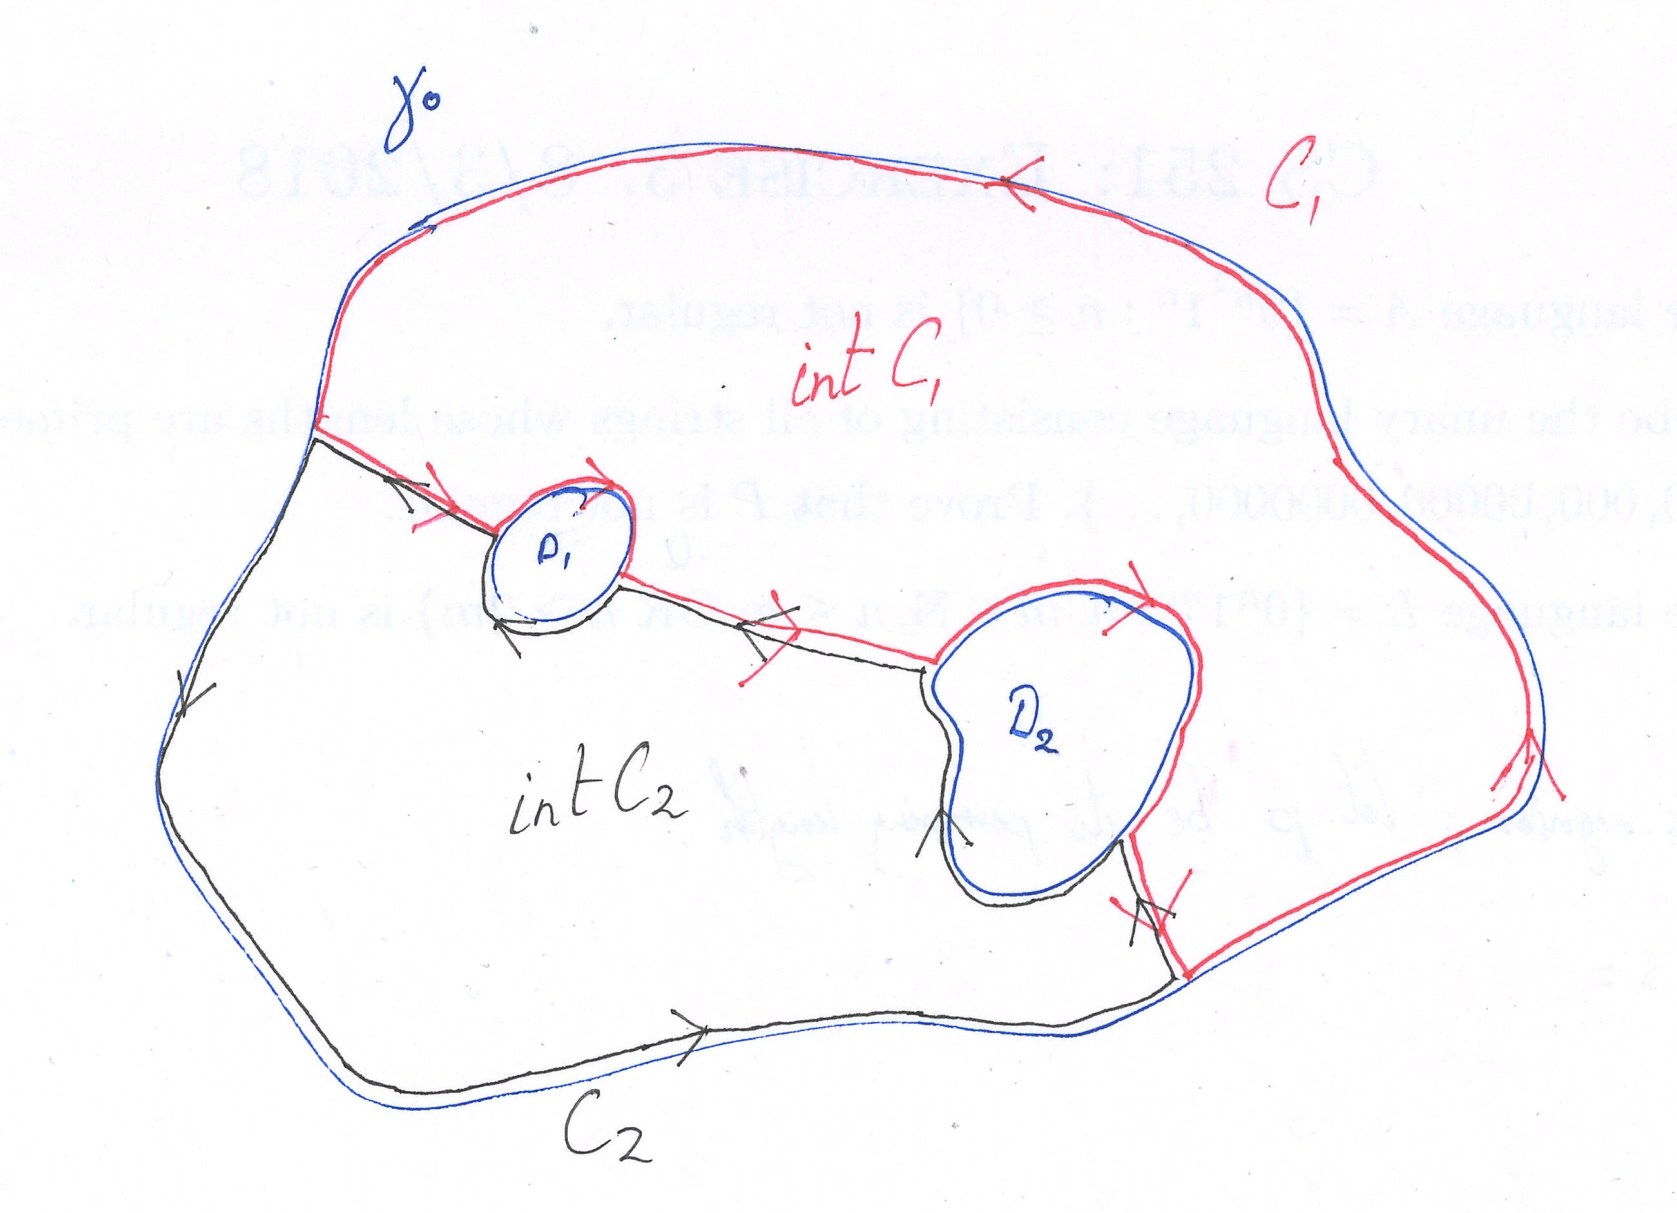
\includegraphics[width=.65\linewidth]{img/3_2_4-heur.png}
    \caption{Illustration de la justification heuristique}
    \label{3_2_4-heur}
\end{figure}

\[
D = \adh{D_0} \setminus \big(D_1 \cup D_2\big) = \adh{C_1} \cup \adh{C_2}
\]

Les bords de $\gamma_0, \gamma_1$ et $\gamma_2$ de $D_0,D_1$ et $D_2$ appartiennent à $D$.

\begin{itemize}
    \item 
    D'une part, $f$ holomorphe dans $\adh{C_1}$ et $\adh{C_2}$, $C_1$ et $C_2$ sont fermés $\xRightarrow[\textrm{Cauchy}]{\textrm{Thm.}}$
    
    \[\int_{C_1} f(z) \dz = 0 \textrm{ et } \int_{C_2} f(z) \dz = 0\]
    \item 
    D'autre part, avec $C_1$ et $C_2$ orientés positivement, on a:
    
    \[
    \int_{C_1} f(z) \dz + \int_{C_2} f(z) \dz = \int_{\gamma_0} f(z) \dz + \int_{\gamma_1} f(z) \dz + \int_{\gamma_2} f(z) \dz
    \]
    
    où $\gamma_0$ est orientée \textit{positivement} ($D_0$ à gauche), mais $\gamma_1$ et $\gamma_2$ orientées \textit{négativement} ($D_1$ et $D_2$ à droite).
\end{itemize}

Donc:

\[\int_{\gamma_0} f(z) \dz + \int_{\gamma_1} f(z) \dz + \int_{\gamma_2} f(z) \dz = 0\]

\begin{align*}
\implies \int_{\gamma_0} f(z) \dz &= - \int_{\gamma_1} f(z) \dz - \int_{\gamma_2} f(z) \dz \quad \textrm{orientation négative (dessin)}\\
&= \int_{\gamma_1} f(z) \dz + \int_{\gamma_2} f(z) \dz \quad \textrm{orientation positive (énoncé)}
\end{align*}


\section{Formule intégrale de Cauchy}

\subsection{Énoncé}

\begin{theorem}
    Soient $D \subset \C$ un domaine simplement connexe, $f: D \rightarrow \C$ une fonction holomorphe dans $D$ et $\gamma$ une courbe simple fermée régulière (par morceaux) orientée positivement contenue dans $D$.
    Alors:
    
    \[
    f(z) = \oipi \int_\gamma \frac{f(\xi)}{\xi - z} \dxi \quad \forall z \in \inte \gamma
    \]
\end{theorem}

\begin{illustration}
    $D = \C$
    
    Si $f$ est une fonction holomorphe dans $\C$, la valeur de la fonction $f$ en un point $z \in \C$ s'obtient en intégrant $\frac{f(\xi)}{\xi - z}$ le long de n'importe quelle courbe $\gamma$ (orientée positivement) telle que $z \in \inte \gamma$.
\end{illustration}

\subsection{Exemples d'utilisation}

\begin{example}[1]
    Soit $\gamma$ une courbe simple fermée régulière.
    Discuter en fonction de $\gamma$ la valeur de l'intégrale:
    
    \[\int_\gamma \frac{\cos 2z}{z} \dz\]
    
    Constatation: la fonction $g(z) = \frac{\cos 2z}{z}$ n'est pas définie en $z = 0$.
    
    Distinction de différents cas:
    
    \begin{description}
    \item[1\ier{} cas $0 \in \gamma$]
    L'intégrale n'est pas définie puisque $g(z) = \frac{\cos 2z}{z}$ n'est pas continue sur $\gamma$.
    
    \item[2\ieme{} cas $0 \notin \adh{\gamma}$]
    La fonction $g(z) = \frac{\cos 2z}{z}$ est holomorphe dans un domaine $D$ simplement connexe tel que $\adh{\gamma} \subset D$.
    Comme $\gamma \subset \adh{\gamma} \subset D$, alors le Thm. de Cauchy s'applique à la fonction $g$ et on trouve:
    
    \[\int_\gamma \frac{\cos 2z}{z} \dz = 0\]
    
    $\forall \gamma$ de ce type (i.e. $0 \notin \adh{\gamma}$).
    
    \item[3\ieme{} cas $0 \in \inte{\gamma}$]
    La fonction $f(\xi) = \cos 2\xi$ est holomorphe dans $\C$.
    Comme $\gamma \subset \C$, en lui appliquant la formule intégrale de Cauchy pour $z = 0$ (avec $D = \C$), on trouve:
    
    \[
    f(0) = \oipi \int_\gamma \frac{\cos 2\xi}{\xi - 0} \dxi
    \implies \int_\gamma \frac{\cos 2\xi}{\xi} \dxi = 2\pi i f(0) = 2\pi i \cos 0 = 2\pi i
    \]
    
    \textbf{Conclusion:} $\int_\gamma \frac{\cos 2z}{z} \dz = 2\pi i \quad \forall \gamma$ de ce type.
    \end{description}
\end{example}

\begin{remark}
    Pour le cercle unité de rayon $1$, on a $\gamma(\theta) = e^{i\theta}$ avec $\theta \in [0,2\pi[$, il faudrait calculer:
    
    \[
    \int_\gamma \frac{\cos 2z}{z} \dz
    = \int_0^{2\pi} \frac{\cos \big(2e^{i\theta}\big)}{e^{i\theta}} i e^{i\theta} \dth
    = i \int_0^{2\pi} \cos \big(2e^{i\theta}\big) \dth
    \]
\end{remark}

\begin{example}[2]
    Calculer
    
    \[\int_\gamma \frac{e^{z^2}}{z + i\pi} \dz\]
    
    où $\gamma$ est le cercle de rayon $4$ centré en $z = 1$.
    
    Utilisation de la formule de Cauchy, constatations:
    
    \begin{enumerate}[label=\arabic{enumi})]
    \item 
    La fonction $g(z) = \frac{e^{z^2}}{z + i\pi}$ n'est pas définie en $z = -i\pi$
    \item 
    $-i\pi \in \inte{\gamma}$
    \end{enumerate}

    On considère $\gamma$ orientée positivement et $f(\xi) = e^{\xi^2}$ qui est holomorphe dans $\C$.
    Formule intégrale de Cauchy pour $z = -i\pi$ (avec $D = \C$) donne:
    
    \[
    f(-i\pi) = \oipi \int_\gamma \frac{e^{\xi^2}}{\xi + i\pi} \dxi \implies \int_\gamma \frac{e^{\xi^2}}{\xi + i\pi} \dxi = 2\pi i f(-i\pi)
    \]
    
    Mais $f(-i\pi) = e^{(-i\pi)^2} = e^{-\pi^2}$, donc:
    
    \[\int_\gamma \frac{e^{z^2}}{z + i\pi} \dz = 2\pi i e^{-\pi^2}\]
    
    \textit{Autres exemples: ex. 1-4, série 6}
\end{example}

% 3.3.3
\subsection{Démonstration de la formule intégrale de Cauchy}

\begin{proof}
Soit $f$ holomorphe dans $D$ et $\gamma$ une courbe simple fermée régulière orientée positivement et contenue dans $D$.
Soient $z \in \inte \gamma$ et $C$ un cercle de rayon $r$ centré en $z$ orienté positivement tel que $C \subset \inte \gamma$.
On note $V = \adh{\gamma} \setminus \inte C$.

Corollaire du Thm. de Cauchy (§3.2.4) appliqué à la fonction $g(\xi) = \frac{f(\xi)}{\xi - z}$ holomorphe pour $\xi \in V$ 

\begin{align*}
\implies \int_\gamma \frac{f(\xi)}{\xi - z} \dxi
&\overset{\textrm{Cor.}}{\underset{\textrm{Thm. Cauchy}}{=}}
\int_C \frac{f(\xi)}{\xi - z} \dxi
\overset{\ast}{=}
\int_0^{2\pi} \frac{f(z + re^{i\theta})}{re^{i\theta}}ire^{i\theta} \dth
\\&=
i \int_0^{2\pi} f(z + re^{i\theta}) \dth
\end{align*}

\[^\ast \xi(\theta) = z + re^{i\theta},
\quad \theta \in [0, 2\pi[,
\quad \xi'(\theta) = ire^{i\theta}\]

D'une part, on a:

\[
\lim_{r \rightarrow 0} \int_\gamma \frac{f(\xi)}{\xi - z} \dxi = \int_\gamma \frac{f(\xi)}{\xi - z} \dxi \ \textrm{(grandeur indépendante de $r$)}
\]

D'autre part, on a:

\begin{align*}
\lim_{r \rightarrow 0} \int_0^{2\pi} f(z + re^{i\theta}) \dth &=
\int_0^{2\pi} \lim_{r \rightarrow 0} \big[f(z + re^{i\theta})\big] \dth
\overset{f \ \textrm{continue}}{=}
\int_0^{2\pi} f(z) \dth
\\&=
f(z) \int_0^{2\pi} \dth
= 2\pi f(z)
\end{align*}

Égalité des limites:

\[\implies \int_\gamma \frac{f(\xi)}{\xi - z} \dxi = 2\pi i f(z)\]
\end{proof}

% 3.4
\section{Corollaire de la formule intégrale de Cauchy}

\subsection{Énoncé}

Avec les mêmes hypothèses du §3.3 ($D \subset \C$ domaine simplement connexe, $f: D \rightarrow \C$ holomorphe dans $D$, $\gamma \subset D$ courbe fermée régulière orientée positivement), on a:

\begin{enumerate}[label=\arabic{enumi})]
    \item 
    $f$ est infiniment dérivable dans $D$
    \item 
    \[
    f^{(n)}(z) = \frac{n!}{2\pi i} \int_\gamma \frac{f(\xi)}{(\xi - z)^{n+1}} \dxi \quad \textrm{pour } n \in \N, \ \forall z \in \inte \gamma
    \]
\end{enumerate}

Commentaires

\begin{enumerate}[label=\arabic{enumi})]
    \item 
    Pour $n=0$, le corollaire redonne la formule intégrale de Cauchy:
    
    \[
    f(z) = f^{(0)}(z) = \frac{0!}{2\pi i} \int_\gamma \frac{f(\xi)}{\xi - z} \dxi
    \]
    
    \item 
    Résultat remarquable: le corollaire affirme qu'une fonction holomorphe dans $D$ (i.e. dérivable $\forall z \in D$) est en fait infiniment dérivable et que sa $n$-ième dérivée se calcule en dérivant $n$ fois par rapport à $z$ sous l'intégrale de la formule de Cauchy.
    En effet: $\quad ' = \frac{\dd}{\dz}$
    
    \[
    f^{(1)}(z) = \frac{1}{2\pi i} \int_\gamma f(\xi) \left[\frac{1}{\xi - z}\right]' \dxi
    = \frac{1}{2\pi i} \int_\gamma \frac{f(\xi)}{(\xi - z)^2} \dxi = \frac{1!}{2\pi i} \int_\gamma \frac{f(\xi)}{(\xi - z)^2} \dxi
    \]
    
    \[
    f^{(2)}(z) = \frac{1}{2\pi i} \int_\gamma f(\xi) \left[\frac{1}{(\xi - z)^2}\right]' \dxi
    = \frac{2}{2\pi i} \int_\gamma \frac{f(\xi)}{(\xi - z)^3} \dxi = \frac{2!}{2\pi i} \int_\gamma \frac{f(\xi)}{(\xi - z)^3} \dxi 
    \]
    
    \[
    f^{(3)}(z) = \frac{2}{2\pi i} \int_\gamma f(\xi) \left[\frac{1}{(\xi - z)^3}\right]' \dxi
    = \frac{2 \cd 3}{2\pi i} \int_\gamma \frac{f(\xi)}{(\xi - z)^4} \dxi = \frac{3!}{2\pi i} \int_\gamma \frac{f(\xi)}{(\xi - z)^4} \dxi 
    \]
    
    Récurrence sur $n$:
    
    \[
    f^{(n)}(z) = \frac{n!}{2\pi i} \int_\gamma \frac{f(\xi)}{(\xi - z)^{n+1}} \dxi
    \]
\end{enumerate}

\subsection{Exemples d'utilisation}

\begin{example}[1]
    Calculer:
    
    \[
    \int_\gamma \frac{z e^{3z + 5}}{(z + 1)^3}\dz \ \textrm{ où }\ \gamma = \big\{z \in \C : \module{z - i} = 2\big\}
    \]
    
    Constatations:
    
    \begin{enumerate}[label=\arabic{enumi})]
    \item 
    la fonction $g(z) = \frac{z e^{3z + 5}}{(z + 1)^3}$ n'est pas définie en $z = -1$
    
    \item 
    $\gamma$ est le cercle de rayon $2$ centré en $z_0 = i$ et $-1 \in \inte \gamma$.
    
    On considère $\gamma$ orientée positivement et la fonction $f(\xi) = \xi e^{3\xi + 5}$ qui est holomorphe dans $\C$.
    \end{enumerate}

    En appliquant à $f$ le corollaire de la formule de Cauchy pour $z = -1$ et $n = 2$ (avec $D = \C$), on obtient:
    
    \[f''(-1) = \frac{2!}{2\pi i} \int_\gamma \frac{\xi e^{3\xi + 5}}{(\xi + 1)^3} \dxi\]
    
    mais $f'(\xi) = \big(\xi e^{3\xi + 5}\big)' = e^{3\xi + 5} + 3 \xi e^{3\xi + 5}$ et $f''(\xi) = 3 e^{3\xi + 5} + 3 e^{3\xi + 5} + 9 \xi e^{3\xi + 5}$
    
    \[ \implies f''(-1) = -3 e^2 \]
    
    \textbf{Donc:}
    
    \[
    \int_\gamma \frac{\xi e^{3\xi + 5}}{(\xi + 1)^3} \dxi
    = -3\pi i e^2
    \]
\end{example}

\begin{example}[2]
    Soit $\gamma$ une courbe simple fermée régulière.
    Discuter en fonction de $\gamma$ la valeur de l'intégrale:
    
    \[\int_\gamma \frac{z^2 \sin z}{2 (z - \frac{\pi}{2})^2} \dz\]
    
    La fonction $g(z) = \frac{z^2 \sin z}{2 (z - \frac{\pi}{2})^2}$ n'est pas définie pour $z = \frac{\pi}{2} \implies$ distinction de plusieurs cas.
    
    \begin{itemize}
        \item \textbf{1\ier{} cas} $\frac{\pi}{2} \in \gamma$
        
        L'intégrale n'est pas définie puisque $g(z) = \frac{z^2 \sin z}{2 (z - \frac{\pi}{2})^2}$ n'est pas continue en $z = \frac{\pi}{2}$
        
        \item \textbf{2\ieme{} cas} $\frac{\pi}{2} \notin \adh{\gamma}$
        
        La fonction $g(z) = \frac{z^2 \sin z}{2 (z - \frac{\pi}{2})^2}$ est holomorphe dans un domaine simplement connexe $D$ tel que $\adh{\gamma} \subset D$. Comme $\gamma \subset \adh{\gamma} \subset D$, alors le Théorème de Cauchy s'applique à $g$ et on trouve:
        
        \[ \int_\gamma \frac{z^2 \sin z}{2 (z - \frac{\pi}{2})^2} \dz = 0 \quad \forall \gamma \textrm{ de ce type} \]
        
        \item \textbf{3\ieme{} cas} $\frac{\pi}{2} \in \inte\gamma$
        
        La fonction $f(\xi) = \frac{\xi^2}{2} \sin \xi$ est holomorphe dans $\C$. Comme $\gamma \subset \C$, en lui appliquant le corollaire de la formule de Cauchy pour $z = \frac{\pi}{2}$ et $n = 1$ (avec $D = \C$), on obtient:
        
        \[
        f'\left(\frac{\pi}{2}\right) = \frac{1!}{2\pi i} \int_\gamma \frac{\frac{\xi^2}{2} \sin \xi}{(\xi - \frac{\pi}{2})^2} \dxi
        \]
        
        mais $f'(\xi) = \big(\frac{\xi^2}{2} \sin \xi\big)' = \frac{2\xi}{2} \sin \xi + \frac{\xi^2}{2} \cos \xi$
        
        \[ \implies f'\left(\frac{\pi}{2}\right) = \frac{\pi}{2} + 0 = \frac{\pi}{2} \]
        
        \textbf{Conclusion:}
        
        \[
        \int_\gamma \frac{z^2 \sin z}{2(z - \frac{\pi}{2})^2} \dz = 2\pi i \frac{\pi}{2} = \pi^2 i
        \]
    \end{itemize}
\end{example}

\textit{Autres exemples: ex. 1-4, série 7}
